%\documentclass[pdflatex,a4paper,10pt]{article}
%\documentclass[a4paper,fleqn,10pt]{jsarticle}
\documentclass[pdflatex, a4paper, 10pt, jadriver=standard]{bxjsarticle}
\setlength{\oddsidemargin}{-10mm}
\setlength{\topmargin}{-19mm}
\setlength{\textheight}{250mm}
\usepackage{graphicx}
\usepackage{hyperref}
\pagestyle{empty}

\begin{document}

    
        {\Large Title: Sample1 document}\newline\newline

    

\section*{\Large Text}

	ANTLR is a powerful parser generator.\par

	It's widely used to build languages, tools, and frameworks.\par

  
\section*{\Large Special symbols, Table}

	%table code
\begin{tabular}{|p{0.5\textwidth}|p{0.5\textwidth}|}\hline

		
			Greek symbols&
			$\alpha$, $\beta$, $\gamma$, ...
		\\\hline
		
			Other symbols&
			
			%table code
caption: arrows, degree sign, ...\newline
\begin{tabular}{|p{0.212\textwidth}|p{0.212\textwidth}|}\hline

				
				
					$\uparrow$, $\downarrow$, $\leftarrow$, $\rightarrow$,$\dagger$, ...&
					360$^\circ$,/,--, ...
				\\\hline
			\end{tabular}

			
		\\\hline
	\end{tabular}
\newline

	
 \section*{\Large Anchor,Image}

	Hiroshige's cat in a window, 19th Century By 
		 \href{https://en.wikipedia.org/wiki/Hiroshige}{Utagawa Hiroshige}
\newline

		 alt: Hiroshige's cat\newline
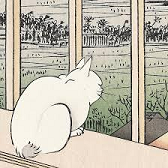
\includegraphics{cat.png}

 
\section*{\Large List}

    
\begin{enumerate}

     \item Food
		 
\begin{itemize}

			  \item Sushi

			  \item Ramen

		
\end{itemize}
	

     \item Drink
		 
\begin{itemize}

			  \item Coffee

			  \item Green Tea

		
\end{itemize}
	

    
\end{enumerate}
    

\end{document}